\documentclass{article}
\usepackage[utf8]{inputenc}
\usepackage[T2A]{fontenc}
\usepackage[russian]{babel}
\usepackage{amsfonts}
\usepackage{amsmath}
\usepackage{amssymb}
\usepackage[left=3cm,right=3cm,top=3cm,bottom=3cm]{geometry}
\usepackage{graphicx}
\usepackage{hyperref}
\usepackage{multicol}
\usepackage{stackrel}
\usepackage{graphicx}
\usepackage{listings}
\usepackage{float}
\usepackage{listings}
\usepackage{inconsolata}
\usepackage{caption}
\usepackage{color}
\usepackage{xcolor}
\DeclareCaptionFont{white}{\color{white}}
\DeclareCaptionFormat{listing}{\colorbox{gray}{\parbox{\textwidth}{#1#2#3}}}
\captionsetup[lstlisting]{format=listing,labelfont=white,textfont=white}
\lstset { %
	language=C++,
	backgroundcolor=\color{white!5},
	tabsize=3,
	basicstyle=\normalsize\fontfamily{zi4}\selectfont,
	literate={\ \ }{{\ }}1
}
\graphicspath{ {./images/} }
\providecommand{\myceil}[1]{\left \lceil #1 \right \rceil }
\begin{document}
	\pagestyle{empty}
	\normalsize
	\newcommand{\R}{{\mathbb R}}
	\newcommand{\N}{{\mathbb N}}
	\newcommand{\lm}[2]{\displaystyle \lim_{#2 \to \infty}{#1_{#2}}}
	\newcommand{\eps}{\varepsilon}
	\section{}
	\begin{center}
\begin{tabular}{ |c|c|c| } 
	\hline
	Лабораторная работа №4 & М3137 & 2023 \\ 
	\hline
	OpenMP & Сологуб Матвей Андреевич & \\ 
	\hline
\end{tabular}
\end{center}
	\large
	\section{}
\paragraph{Цель работы:}
Знакомство с основами многопоточного программирования.
\paragraph{Инструментарий:}
Microsoft Visual C++20 / GNU C++20 с OpenMP.
\section{OpenMP}
OpenMP - минималистичная библиотека для распараллеливания вычислений, включает в себя следующие конструкции:
\paragraph{\textcolor{gray}{\textit{\LARGE{\#pragma omp parallel}}}}
Создаёт некоторое количество тредов. Весь код который помещён внутрь этого блока будет параллельно исполняться в каждом из тредов. Можно явно указать сколько потоков мы хотим использовать при помощи num\_threads(число потоков), однако это может изменить лишь верхнюю границу. Сколько потоков будет использоваться на самом деле зависит как от реального количества доступных тредов, так и от того сколько нам их выделит ОС.
\paragraph{\textcolor{gray}{\textit{\LARGE{\#pragma omp critical}}}}
Если мы хотим чтобы код выполняемый внутри параллельного региона взаимодействовал с памятью, доступной всем потокам (общей), нам следует быть очень осторожными. Когда мы пишем в память в однопоточной программе, мы знаем что она принадлежит нам и никто другой с ней взаимодействовать не может. Когда же у нас есть несколько потоков, они могут менять/читать одну и ту же память одновременно, что приведёт к \textbf{race condition}. Переменные объявленные внутри параллельного региона свои у каждого потока, так что их можно изменять как обычно. А для работы с общедоступными переменными следует использовать блок \textbf{critical}. Он даёт гарантию того, что код помещённый в него в любой момент времени будет исполняться лишь одним потоком. Несложно догадаться, что это может привести к падению производительности, ведь когда один из потоков выполняет этот код, потоки которые тоже должны его выполнить простаивают без дела.
\paragraph{\textcolor{gray}{\textit{\LARGE{\#pragma omp for}}}}
Автоматически распределяет итерации цикла между потоками (должен объявляться внутри параллельного региона, или же, вместе с ним \textbf{\#pragma omp parallel for}). То - как именно будут распределенеы итерации определяет \textbf{schedule(type, chunkSize)} - вид распределения и число итераций в одном чанке (\textbf{chunkSize} - опционально). \textbf{static} - все потоки получают одинаковое число chunk-ов, в каждом из них \textbf{chunkSize} итераций. Используется когда на каждой итерации выполняется примерно одинаковое количество работы, так как тогда все треды будут одинаково загружены. \textbf{dynamic} - во время работы создаётся очередь, из которой свободные потоки берут себе на выполнение чанки итераций. Используется когда разные итерации имеют различное количество работы. Если использовать в такой ситуации \textbf{static}, треды которым попались тяжёлые чанки всё время были бы загружены, а те которым попались лёгкие в этом время будут простаивать. С \textbf{dynamic} такой проблемы не возникает, так как когда какой-то тред освобождается он сразу берёт новый чанк из очереди. Но конечно все эти дополнительные вычисления происходят в рантайме и не бесплатны.
\paragraph{\textcolor{gray}{\textit{\LARGE{\#pragma omp barrier}}}}
Всё что делает - заставляет потоки дошедшие до этого барьера ждать, пока до него дойдут остальные и лишь потом продолжать выполнение. Полезно когда необходимо чтобы какой-то фрагмент кода выполнялся лишь тогда, когда всё что есть до него уже полностью посчитано. Неявно используется в конце \textbf{\#pragma omp parallel} и \textbf{\#pragma omp for}, но во втором случае его можно отключить с помощью ключевого слова nowait, тогда потоки завершившие выполнение цикла не будут дожидаться остальных, что может улучшить производительность, однако нужно быть уверенным что никаких конфликтов из-за этого не возникнет.
\paragraph{\textcolor{gray}{\textit{\LARGE{\#pragma omp single}}}}
Используется внутри параллельного региона, говорит исполнять указанный код лишь одним тредом. В конце неявный барьер.
\paragraph{\textcolor{gray}{\textit{\LARGE{\#pragma omp atomic}}}}
Более быстрая версия \textbf{critical}, но лишь на одну из поддерживыемых \textbf{атомарных} операций. Например, удобно обновлять какой-нибудь общий счётчик. Не использовал.
\paragraph{\textcolor{gray}{\textit{\LARGE{Lock}}}}
Ещё более низкоуровневая концепция, так же используется для синхронизации тредов. Позволяет создать \textbf{omp\_lock\_t} инициализировать его с помощью \textbf{omp\_init\_lock(\&lock)}, и на время пользования какой-либо памятью поставить его в \textbf{omp\_set\_lock}, а по окончании вернуть \textbf{omp\_unset\_lock}. Тогда другие треды смогут с помощью \textbf{omp\_test\_lock} узнать его статус и пока доступа к нужной им памяти у них нет заняться чем-то другим, а не просто ждать.

\section{Описание кода}

Парсим аргументы командной строки, проверяем на корректность. Читаем файл методом \textbf{parse}, проверяем что первая строка - P5, далее два целых положительных числа - длина и высота изображения и число 255 - наибольший оттенок. Считываем файл в массив  \textbf{data} из $width*height$ байт. Отсюда начинается отсчёт времени работы алгоритма и параллельный регион. Считаем гистограмму $histo[256]$, где \textbf{$histo_i$} - число пикселей яркости $i$ в картине. Подсчёт гистограммы я тоже решил распараллелить, так как в случае больших картинок это может стать узким горлышком. Каждый тред обрабатывает только часть картинки и считает гистограмму для этой части, а затем в секторе \textbf{critical} эти гистограммы складываются в одну. Используем $for$ со $schedule(static, 1)$, так как все итерации имеют одинаковую сложность и в конце ставим барьер, так как дальше мы будем ипользовать гистограмму.
\begin{lstlisting}[label=histo-calc,caption=Подсчёт гистограммы]
int lHisto[256]{};
#pragma omp for schedule(static)
for (int i = 0; i < pixelsNum; ++i) {
	++lHisto[data[i]];
}
#pragma omp critical
{
	for (int i = 0; i < 256; ++i) {
		histo[i] += lHisto[i];
	}
}
#pragma omp barrier
\end{lstlisting}
Сперва, я реализовал подсчёт гистограммы не через \textbf{critical}, а через \textbf{lock'и}, имея одну общую гистограмму и обновляя её в каждом треде предварительно залочив обновляемую ячейку. Но такое решение было на порядок медленнее того, которое я описал ранее. Я думаю, это вызвано тем, что оттенков всего 256 и довольно часто случались коллизии которые вызывали простой тредов. Однако в случае если бы у нас была \textbf{RGB} картинка, кажется, это решение было бы оптимальным.\\Теперь сам алгоритм: полным перебором ищем три порога - три вложенных цикла. На каждой итерации внутреннего цикла считаем межклассовую дисперсию и запоминаем комбинацию порогов на которой она максимальна (Можно было бы минимизировать дисперсию внутри класса, но сделать это быстро нельзя, а Оцу как раз показал, что минимизация внутриклассовой дисперсии эквивалента максимизации межклассовой, которая в свою очередь находится элементарно).  Но перед началом самого цикла сделаем некоторый предподсчёт в регионе $single$. Для пересчёта дисперсии мы хотим как можно быстрее отвечать на следующие запросы: число пикселей с яркостью $[l ; r]$ и сумма яркостей пикселей с яркостью $[l ; r]$. Для этого посчитаем два префиксных массива $histoNumPrefixes$ и $histoBrightPrefixes$. Создаём переменные $lMaxDisp = 0, lF0, lF1, lF2$ - максимальная дисперсия полученная в данном треде и соответствующии ей пороги.
\begin{lstlisting}[label=precalc,caption=Предподсчёт]
#pragma omp single
{
	for (int i = 1; i < 257; ++i) {
		histoNumPrefixes[i] = histoNumPrefixes[i - 1] + histo[i - 1];
		histoBrightPrefixes[i] = histoBrightPrefixes[i - 1] + histo[i - 1] * (i - 1);
		if (histo[i-1] && minBrightness > i-1){
			minBrightness = i-1;
		}
		if (histo[i-1] && maxBrightness < i-1){
			maxBrightness = i-1;
		}
	}
}
\end{lstlisting}
 Теперь сами циклы: используем $for$ со $schedule(dynamic)$ так как разные итерации цикла сильно разнятся по сложности, а именно с увеличением $f0$ сложность сильно падает, так как вложенные циклы делают меньше итераций. В первом цикле будем выбирать значение первого порога, во втором начиная со значения первого + 1 будем выбирать второй порог, и в третьем аналогично. В начале каждого цикла сделаем проверку на то, есть ли вообще пиксели с яркостью этого порога. Если таких пикселей нет, то итерацию можно пропустить, так как если полученная дисперсия и будет максимальной, то она либо уже встречалась до этого, либо встретится после. Можно было бы проверять это как просто $histo_f == 0$, но так как больше обращений к $histo$ мы делать не будем, лучше проверять $histoNumPrefixes[f+1] == histoNumPrefixes[f]$, сэкономим место в кэше. Такая оптимизация может дать значительный выигрышь в скорости лишь на картинках которые содержат не все цвета, однако такие картинки довольно часто встречаются, так что она вполне оправдана. Далее рассмотрим последний внутренний цикл: в нём мы и будем вычислять межклассовую дисперсию. Заведём переменную $disp$ типа \textbf{double}, в ней будет храниться дисперсия для текущих порогов, которая считается по следующей формуле: $\sigma^2 = \displaystyle\sum_{i=1} ^{4}cProb*cAvgBrightness^2$, где $cProb$ это число пикселей попадающих в кластер поделённое на общее число пикселей, а $cAvgBrightness$ это средняя яркость пикселей в кластере, которая равна сумме яркостей пикселей в кластере поделённой на их число. Эти величины мы можем найти из нашего массива префиксных сумм. Проходим в цикле по 4-м кластерам и прибавляем полученное значение к общей сумме $disp$. В случае если $disp \geq lMaxDisp$ обновляем $lMaxDisp$ и пороги текущими значениями. После циклов в секции \textbf{critical} обновляем общие $maxDisp$ и порог. Ставим барьер - нам необходимо чтобы все треды закончили подсчёт максимальной дисперсии и обновили её.
\begin{lstlisting}[label=algo,caption=Поиск наилучших порогов]
double lMaxDisp = 0;
int lF0 = -1, lF1 = -1, lF2 = -1;
#pragma omp for schedule(dynamic)
for (int f0 = 0; f0 <= maxBrightness; ++f0) {
	if (histoNumPrefixes[f0 + 1] == histoNumPrefixes[f0])
	continue;
	for (int f1 = f0 + 1; f1 <= maxBrightness; ++f1) {
		if (histoNumPrefixes[f1 + 1] == histoNumPrefixes[f1])
		continue;
		for (int f2 = f1 + 1; f2 <= maxBrightness; ++f2) {
			if (histoNumPrefixes[f2 + 1] == histoNumPrefixes[f2])
			continue;
			double disp = 0;
			for (int i = 0; i < clustersCount; ++i) {
				int l, r;
				if (i == 0) {
					l = minBrightness, r = f0;
				}
				else if (i == 1) {
					l = f0 + 1, r = f1;
				}
				else if (i == 2) {
					l = f1 + 1, r = f2;
				}
				else {
					l = f2 + 1, r = maxBrightness;
				}
				int cPixelsNum = histoNumPrefixes[r + 1] - histoNumPrefixes[l];
				int cBrightSum = histoBrightPrefixes[r + 1] - histoBrightPrefixes[l];
				double cProb = (double)cPixelsNum / pixelsNum;
				double cAvgBrightness = (double)cBrightSum / cPixelsNum;
				disp += cProb * cAvgBrightness * cAvgBrightness;
			}
			if (disp >= lMaxDisp) {
				lMaxDisp = disp;
				lF0 = f0, lF1 = f1, lF2 = f2;
			}
		}
	}
}
#pragma omp critical
{
	if (lMaxDisp >= maxDisp) {
		maxDisp = lMaxDisp;
		F0 = lF0, F1 = lF1, F2 = lF2;
	}
}
#pragma omp barrier
\end{lstlisting}
  Далее фильтруем картинку - каждый тред некоторую её часть, используя $schedule(static)$, так как все итерации цикла одинаковы по сложности.
  \begin{lstlisting}[label=filtr,caption=Фильтрация картинки]
#pragma omp for schedule(static)
for (int i = 0; i < width * height; ++i) {
	if (data[i] <= F0) {
		data[i] = 0;
	}
	else if (data[i] <= F1) {
		data[i] = 84;
	}
	else if (data[i] <= F2) {
		data[i] = 170;
	}
	else {
		data[i] = 255;
	}
}
  \end{lstlisting}
  Завершаем параллельный регион и заканчиваем подсчёт времени. Записываем атрибуты картинки и изменённый массив $data$ в выходной файл.
  \paragraph{Пояснения к коду}
  Я старался писать код так, чтобы компилятору/процессору было легче распараллелить инструкции (\textit{Instruction-level parallelism}). Например распологал независимые друг от друга вычисления поближе. Тем не менее, кажется, что большую часть таких оптимизаций современные компиляторы и сами сделают, если не написать какую-нибудь совсем уж откровенную фигню. Ну и не буду ведь я разворачивать циклы руками! Вам ведь этот код ещё читать.\\
  Также я не параллелил подсчёт массивов префиксных сумм. Во первых, не очень понятно как это можно было сделать (возможно даже никак), а во вторых, по времени эти вычисления занимают даже меньше чем погрешность(256 итераций довольно простого цикла).
  \section{Результат работы}
  Time (12 thread(s)): 5.7168 ms\\
  77 130 187
  \begin{figure}[H]
  	
\includegraphics[width=1\textwidth]{pictures/in1.png}
  	\caption{Лена}
  \end{figure}
  \begin{figure}[H]
  	
\includegraphics[width=1\textwidth]{pictures/out1.png}
  	\caption{Результат работы на Лене}
  \end{figure}
	Time (12 thread(s)): 10.0114 ms \newline
	\quad 32 81 165
  \begin{figure}[H]
	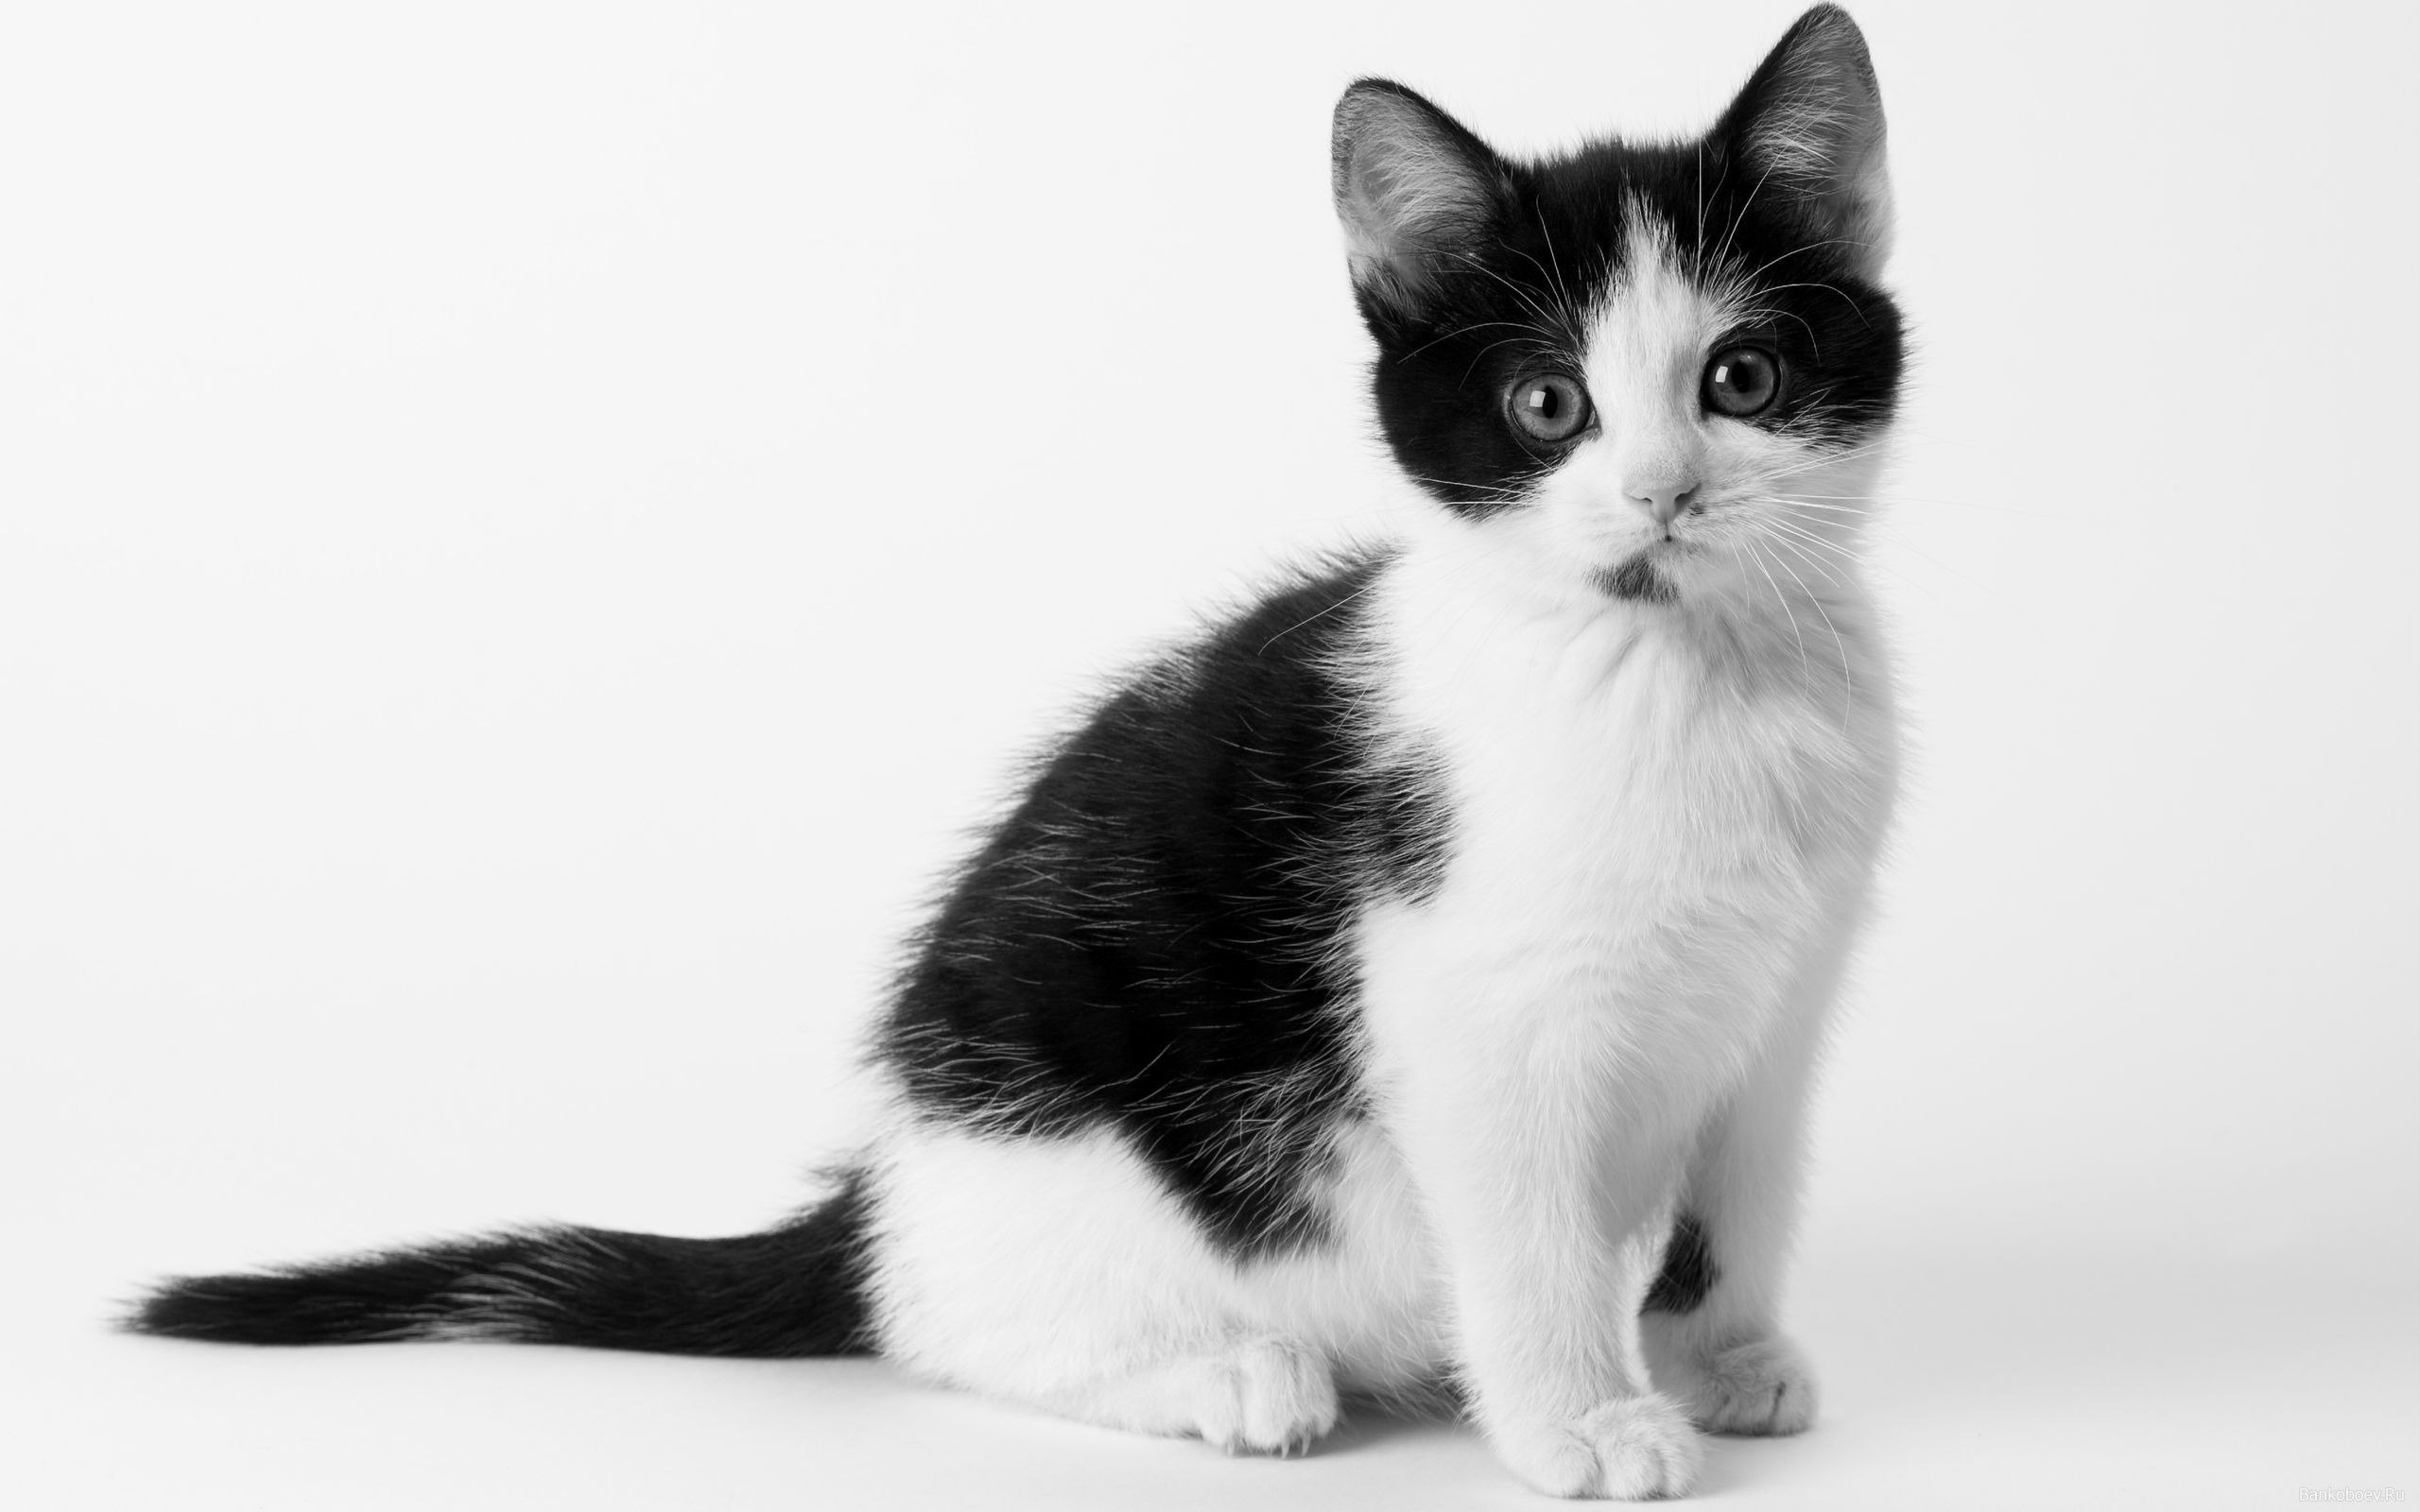
\includegraphics[width=1\textwidth]{pictures/in2.jpg}
	\caption{Большой котик}
  \end{figure}
  \begin{figure}[H]
	
\includegraphics[width=1\textwidth]{pictures/out2.jpg}
	\caption{Результат работы на большом котике}
  \end{figure}
\section{Замеры}
  \begin{figure}[H]
	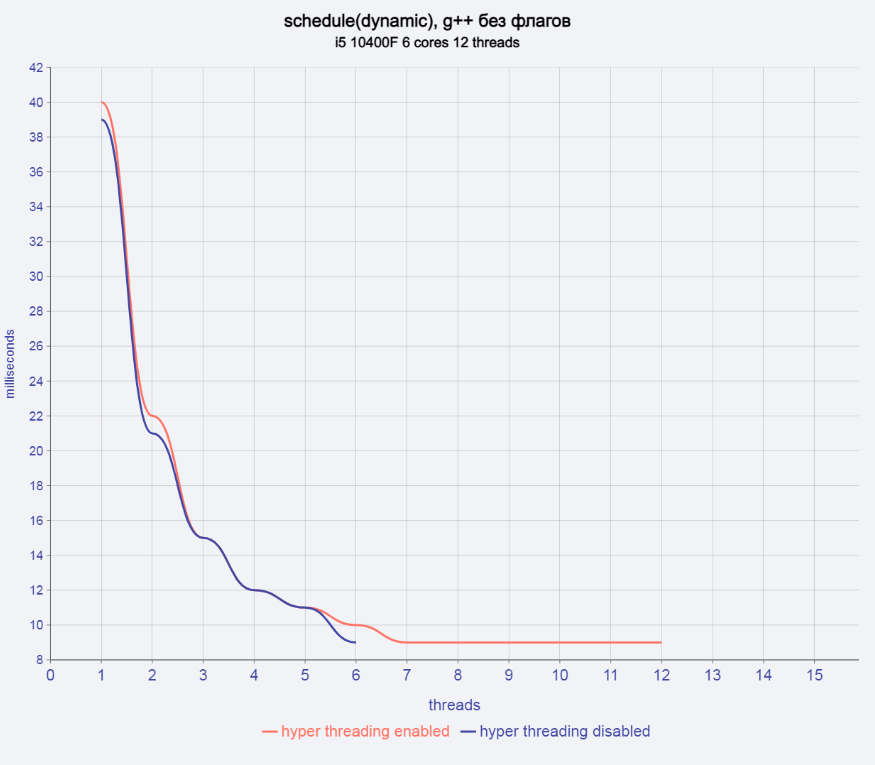
\includegraphics[width=1\textwidth]{pictures/Screenshot_1.png}
	\caption{schedule(dynamic)}
  \end{figure}
  \begin{figure}[H]
	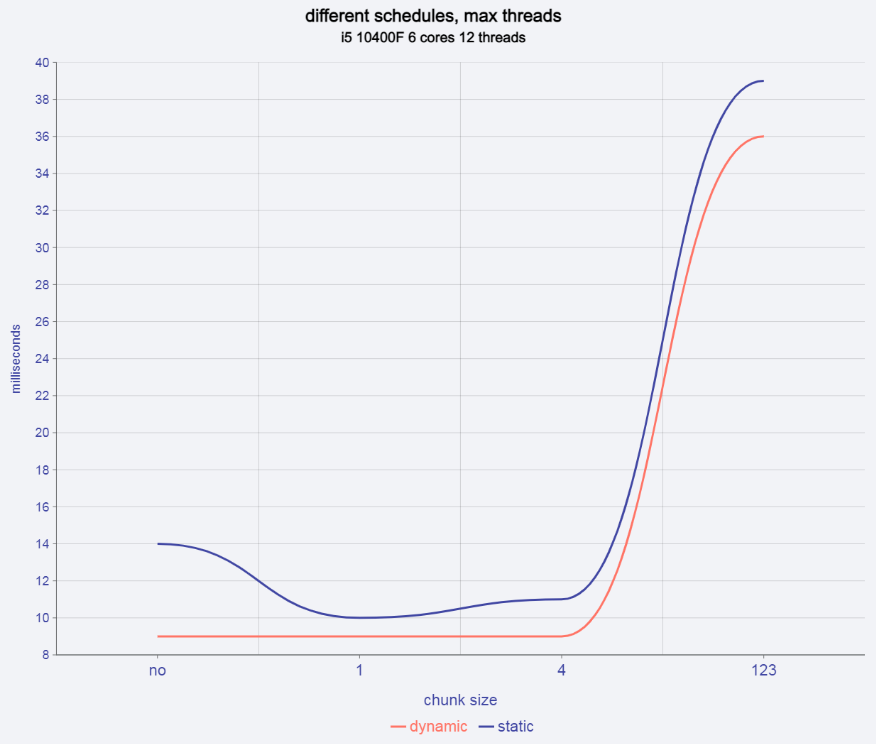
\includegraphics[width=1\textwidth]{pictures/Screenshot_2.png}
	\caption{разные schedule вычисления порогов (общее время)}
  \end{figure}
  \begin{figure}[H]
	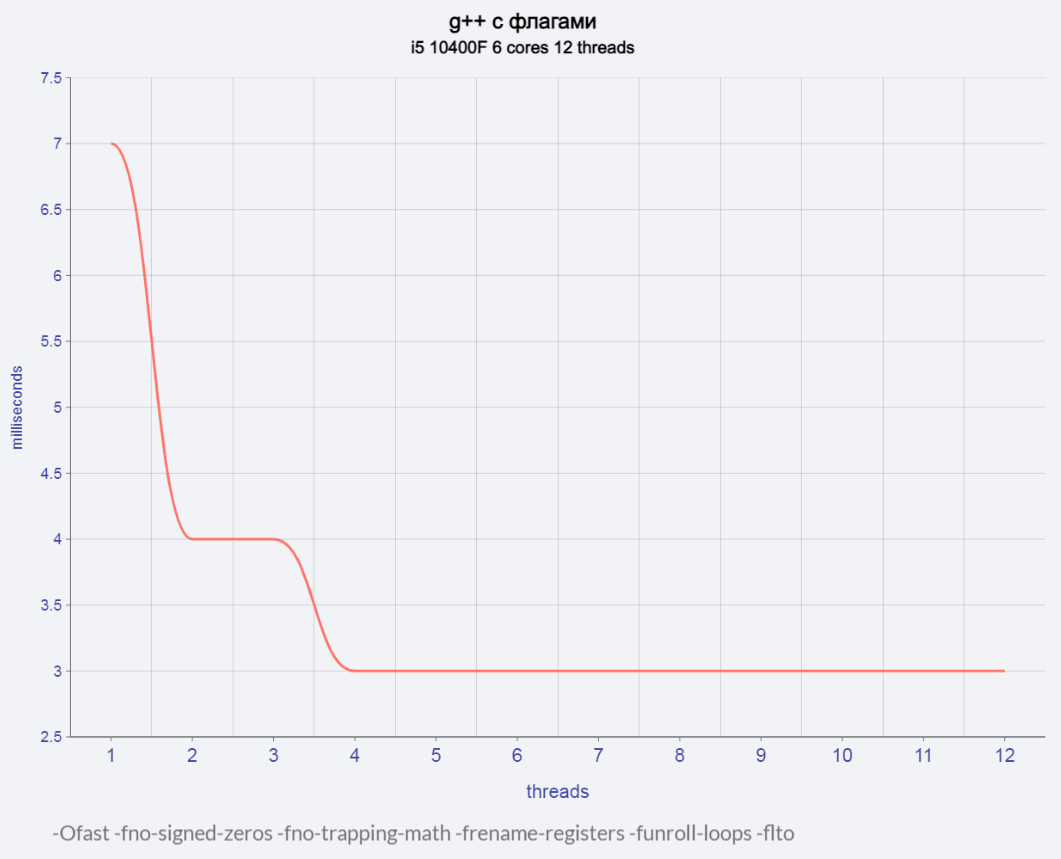
\includegraphics[width=1\textwidth]{pictures/Screenshot_3.png}
	\caption{schedule(dynamic) с флагами оптимизации}
  \end{figure}
  \begin{figure}[H]
	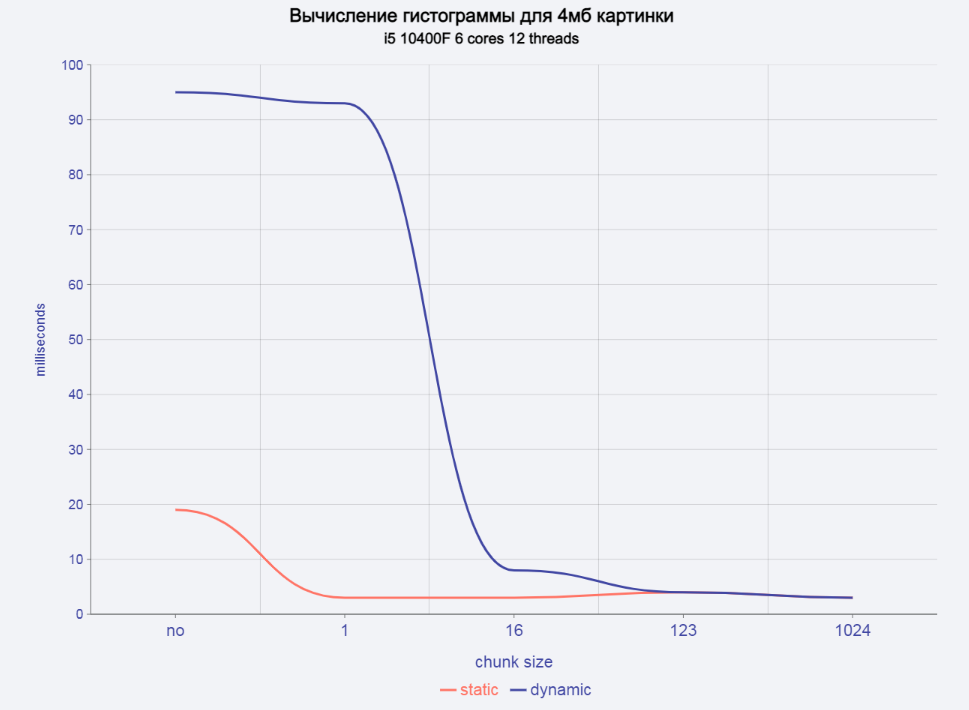
\includegraphics[width=1\textwidth]{pictures/Screenshot_4.png}
	\caption{Разные schedule, только вычисление гистограммы}
  \end{figure}
  \begin{figure}[H]
	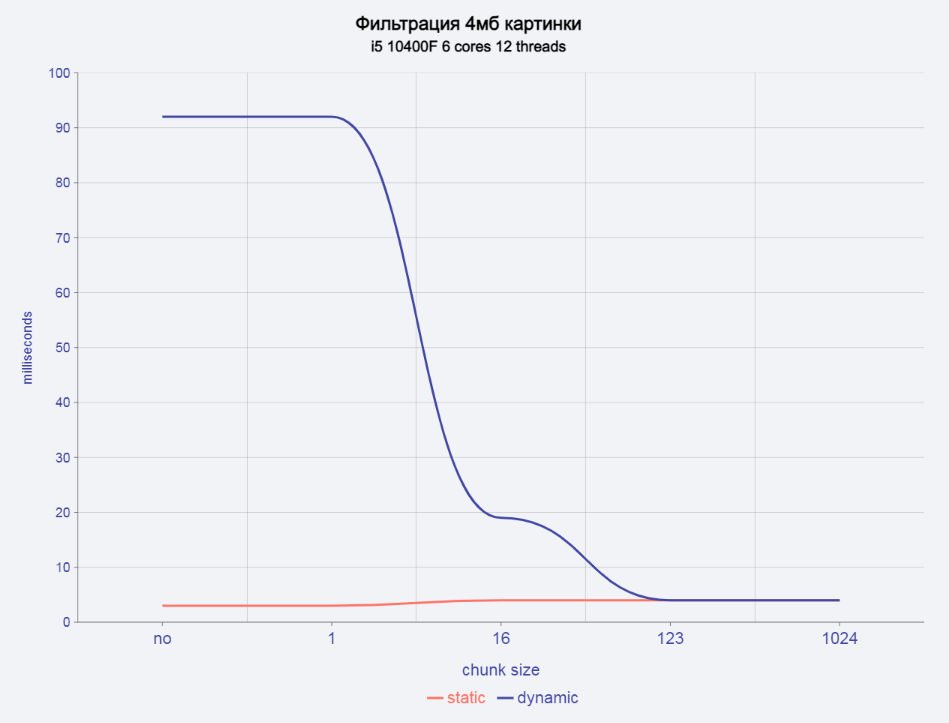
\includegraphics[width=1\textwidth]{pictures/Screenshot_5.png}
	\caption{Только фильтрация картинки}
  \end{figure}
\section{Список источников}
https://wikipedia.tel/Portable\_anymap - про формат pgm\\
https://www.youtube.com/watch?v=nE-xN4Bf8XI - про OpenMP
\section{Листинг кода}
 \begin{lstlisting}[label=list, caption=hard.cpp]
#include <iostream>
#include <omp.h>
#include <vector>
#include <filesystem>
#include <fstream>
#include <string>

constexpr int clustersCount = 4;

inline uintmax_t getFileSize(const std::string& filename) {
	try {
		std::filesystem::path p(filename);
		return std::filesystem::file_size(p);
	}
	catch (std::exception ex) {
		std::cerr << "Unable to get \" " << filename << "\" size\n" << ex.what();
		return 0;
	}
}

inline bool fileExists(const std::string& filename) {
	std::filesystem::path p;
	try {
		p = std::filesystem::path(filename);
	}
	catch (...) {
		return false;
	}
	return std::filesystem::exists(p);
}

inline bool parse(const std::string& fileName, uint8_t*& data, int& width, int& height) {
	std::string fileFormat(3, '\0');
	std::string maxBrightness(4, '\0');
	std::ifstream ifstream;
	try {
		ifstream = std::ifstream(fileName, std::ios_base::binary);
	}
	catch (std::exception& ex) {
		std::cerr << ex.what() << "\nUnable to open input stream from file " << fileName << '\n';
		return false;
	}
	try {
		ifstream >> fileFormat >> width >> height >> maxBrightness;
		ifstream.get();
		if (fileFormat != "P5") {
			std::cerr << "Wrong file format, exptected P5, but got \"" << fileFormat << "\"\n";
		}
		else if (maxBrightness != "255") {
			std::cerr << "Wrong max brightness, exptected 255, but got " << maxBrightness << '\n';
		}
		else if (width <= 0 || height <= 0 || ((long long)width * height > INT32_MAX)) {
			std::cerr << "Invalid dimensions: width: " << width << " height: " << height << '\n';
		}
		else {
			data = reinterpret_cast<uint8_t*>(malloc(width * height));
			ifstream.read(reinterpret_cast<char*>(data), width * height);
			ifstream.close();
			return true;
		}
		ifstream.close();
	}
	catch (std::exception& ex) {
		std::cerr << "Error while reading from " << fileName << '\n' << ex.what() << '\n';
		ifstream.close();
	}
	return false;
}

int main(int argc, char* argv[]) {
	std::vector <std::string> args(argc);
	for (int i = 0; i < argc; i++) {
		args[i] = argv[i];
	}
	if (argc < 4) {
		std::cerr << "Error! Expected 3 arguments but " << std::to_string(args.size() - 1) << " provided";
		return 0;
	}
	std::string inputFileName = args[2];
	std::string outputFileName = args[3];
	int numThreads = omp_get_max_threads();
	bool useOmp = true;
	try {
		int arg1 = std::stoi(args[1]);
		if (arg1 == -1) {
			useOmp = false;
			numThreads = 1;
		}
		else if (arg1 > 0) {
			if (arg1 > omp_get_max_threads()) {
				std::cerr << "Warning! I can only run " << std::to_string(omp_get_max_threads())
				<< " threads, but asked to run " << std::to_string(arg1) << " threads\n";
			}
			numThreads = arg1;
		}
		else if (arg1 < -1) {
			std::cerr << "Incorrect first argument, expected an integer in range[-1, "
			<< std::to_string(omp_get_max_threads()) << "] but got " << args[1] << '\n';
			return 0;
		}
	}
	catch (std::exception& ex) {
		std::cerr << ex.what() << "\nIncorrect first argument, expected an integer in range [-1, "
		<< std::to_string(omp_get_max_threads()) << "] but got " << args[1] << '\n';
		return 0;
	}
	if (!fileExists(inputFileName)) {
		std::cerr << "File \"" << inputFileName << "\" doesn't exists!";
		return 0;
	}
	uintmax_t inputSize = getFileSize(inputFileName);
	uint8_t* data = nullptr;
	int width = 0;
	int height = 0;
	if (!parse(inputFileName, data, width, height)) {
		std::cerr << "Can't parse data, quitting...\n";
		return 0;
	}
	int desiredSize = width * height + std::to_string(width).size() + std::to_string(height).size() + 9;
	if (inputSize != desiredSize) {
		std::cerr << "Error! Expected file size is " << desiredSize << " but actual is " << inputSize << '\n';
		return 0;
	}
	double time0 = omp_get_wtime();
	int pixelsNum = width * height;
	int histo[256]{};
	int histoNumPrefixes[257]{};
	int histoBrightPrefixes[257]{};
	double maxDisp = 0;
	int F0 = -1, F1 = -1, F2 = -1;
	int minBrightness = 255, maxBrightness = 0;
	#pragma omp parallel num_threads(numThreads) if (useOmp)
	{
		int lHisto[256]{};
		#pragma omp for schedule(static)
		for (int i = 0; i < pixelsNum; ++i) {
			++lHisto[data[i]];
		}
		#pragma omp critical
		{
			for (int i = 0; i < 256; ++i) {
				histo[i] += lHisto[i];
			}
		}
		#pragma omp barrier
		#pragma omp single
		{
			for (int i = 1; i < 257; ++i) {
				histoNumPrefixes[i] = histoNumPrefixes[i - 1] + histo[i - 1];
				histoBrightPrefixes[i] = histoBrightPrefixes[i - 1] + histo[i - 1] * (i - 1);
				if (histo[i - 1] && minBrightness > i - 1){
					minBrightness = i - 1;
				}
				if (histo[i - 1] && maxBrightness < i - 1){
					maxBrightness = i - 1;
				}
			}
		}
		double lMaxDisp = 0;
		int lF0 = -1, lF1 = -1, lF2 = -1;
		#pragma omp for schedule(dynamic)
		for (int f0 = 0; f0 <= maxBrightness; ++f0) {
			if (histoNumPrefixes[f0 + 1] == histoNumPrefixes[f0])
			continue;
			for (int f1 = f0 + 1; f1 <= maxBrightness; ++f1) {
				if (histoNumPrefixes[f1 + 1] == histoNumPrefixes[f1])
				continue;
				for (int f2 = f1 + 1; f2 <= maxBrightness; ++f2) {
					if (histoNumPrefixes[f2 + 1] == histoNumPrefixes[f2])
					continue;
					double disp = 0;
					for (int i = 0; i < clustersCount; ++i) {
						int l, r;
						if (i == 0) {
							l = minBrightness, r = f0;
						}
						else if (i == 1) {
							l = f0 + 1, r = f1;
						}
						else if (i == 2) {
							l = f1 + 1, r = f2;
						}
						else {
							l = f2 + 1, r = maxBrightness;
						}
						int cPixelsNum = histoNumPrefixes[r + 1] - histoNumPrefixes[l];
						int cBrightSum = histoBrightPrefixes[r + 1] - histoBrightPrefixes[l];
						double cProb = (double)cPixelsNum / pixelsNum;
						double cAvgBrightness = (double)cBrightSum / cPixelsNum;
						disp += cProb * cAvgBrightness * cAvgBrightness;
					}
					if (disp >= lMaxDisp) {
						lMaxDisp = disp;
						lF0 = f0, lF1 = f1, lF2 = f2;
					}
				}
			}
		}
		#pragma omp critical
		{
			if (lMaxDisp >= maxDisp) {
				maxDisp = lMaxDisp;
				F0 = lF0, F1 = lF1, F2 = lF2;
			}
		}
		#pragma omp barrier
		#pragma omp for schedule(static)
		for (int i = 0; i < width * height; ++i) {
			if (data[i] <= F0) {
				data[i] = 0;
			}
			else if (data[i] <= F1) {
				data[i] = 84;
			}
			else if (data[i] <= F2) {
				data[i] = 170;
			}
			else {
				data[i] = 255;
			}
		}
	}
	double time1 = omp_get_wtime();
	printf("Time (%i thread(s)): %g ms\n%u %u %u\n", numThreads, (time1 - time0) * 1000, F0, F1, F2);
	std::ofstream outputStream;
	try {
		outputStream = std::ofstream(outputFileName, std::ios_base::binary);
	}
	catch (std::exception& ex) {
		std::cerr << "Unable to create output filestream to " << outputFileName << '\n' << ex.what() << '\n';
		return 0;
	}
	try {
		outputStream << "P5\n" << width << ' ' << height << '\n' << "255\n";
		outputStream.write(reinterpret_cast<char*>(data), height * width);
	}
	catch (std::exception& ex) {
		std::cerr << "Error while writing to the " << outputFileName << '\n' << ex.what() << '\n';
		outputStream.close();
		return 0;
	}
	outputStream.close();
}
 	
\end{lstlisting}
\end{document}
